\documentclass[tikz,border=2pt]{standalone}
\usepackage{amsmath,amssymb}
% sans serif for text and math
\renewcommand{\familydefault}{\sfdefault}
\usepackage[eulergreek]{sansmath}
\sansmath
\usepackage{pgfplots}
\pgfplotsset{compat=1.18}
\usetikzlibrary{arrows.meta}
% match the R figures in estimation.qmd
\definecolor{ctrl}{HTML}{1E90FF}  % dodgerblue
\definecolor{trt}{HTML}{FF6A6A}   % indianred1

\begin{document}
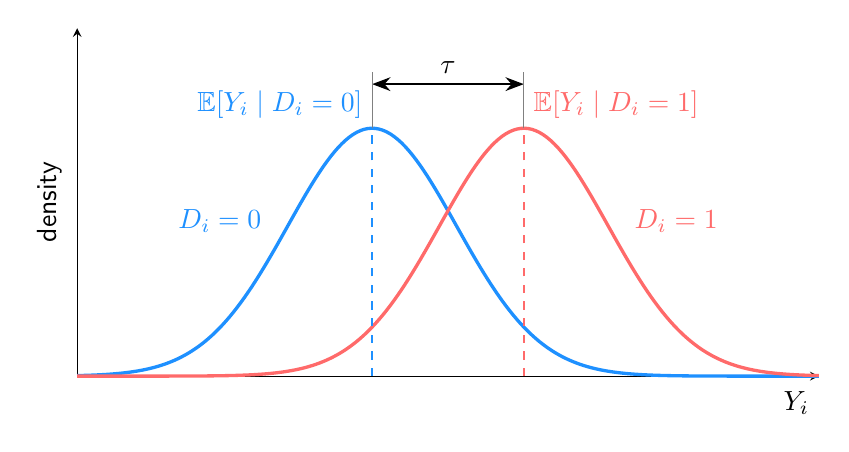
\begin{tikzpicture}[
    declare function={dnorm(\x,\m,\s) = exp(-((\x-\m)^2)/(2*\s^2))/(\s*sqrt(2*pi));}
  ]
  \def\muzero{0}
  \def\muone{1.8}
  \def\sd{1}
  \pgfmathsetmacro{\peak}{dnorm(0,0,\sd)}
  \begin{axis}[
      width=11cm, height=6cm,
      axis lines=left,
      xmin=-3.5, xmax=5.3, ymin=0, ymax=0.56,
      xtick=\empty, ytick=\empty,
      xlabel={$Y_i$}, ylabel={density},
      x label style={at={(axis description cs:1,0)}, anchor=north east, yshift=-2pt},
      clip=false,
    ]
    % densities
    \addplot[ctrl, very thick, domain=-3.5:5.3, samples=200]
      {dnorm(x,\muzero,\sd)};
    \addplot[trt, very thick, domain=-3.5:5.3, samples=200]
      {dnorm(x,\muone,\sd)};
    \node[ctrl, anchor=east] at (axis cs:-1.2,0.25) {$D_i = 0$};
    \node[trt, anchor=west] at (axis cs:3.0,0.25) {$D_i = 1$};

    % means
    \draw[ctrl, thick, dashed] (axis cs:\muzero,0) -- (axis cs:\muzero,\peak);
    \draw[trt, thick, dashed] (axis cs:\muone,0) -- (axis cs:\muone,\peak);
    \node[ctrl, anchor=south east] at (axis cs:\muzero,\peak)
      {$\mathbb{E}[Y_i \mid D_i = 0]$};
    \node[trt, anchor=south west] at (axis cs:\muone,\peak)
      {$\mathbb{E}[Y_i \mid D_i = 1]$};

    % difference
    \draw[{Stealth}-{Stealth}, thick]
      (axis cs:\muzero,0.47) -- node[above] {$\tau$} (axis cs:\muone,0.47);
    \draw[thin, gray] (axis cs:\muzero,\peak) -- (axis cs:\muzero,0.49);
    \draw[thin, gray] (axis cs:\muone,\peak) -- (axis cs:\muone,0.49);
  \end{axis}
\end{tikzpicture}
\end{document}
